\documentclass[11pt,aps,preprint,nofootinbib,superscriptaddress,tightenlines]{revtex4-2}
\usepackage{amsmath,amssymb,bm,mathtools,graphicx}
\usepackage{xcolor}
\definecolor{darkblue}{RGB}{0,0,160}
\usepackage[colorlinks=true,linkcolor=darkblue,citecolor=darkblue,urlcolor=darkblue]{hyperref}

\def\st{\begin{equation}}
\def\stp{\end{equation}}
\def\Eq#1{eq.~(\ref{#1})}
\def\Sect#1{Sect.~\ref{#1}}
\def\Fig#1{Fig.~\ref{#1}}
\newcommand{\avg}[1]{\langle #1\rangle}
\let\oldparagraph\paragraph
\renewcommand{\paragraph}{\par\bigskip\oldparagraph}

\begin{document}

\title{The particle volume from the number density}
\author{D.~Teaney}
\affiliation{Department of Physics and Astronomy, Stony Brook University,
Stony Brook, New York 11794, USA}
\date{\today}

\begin{abstract}
With the energy representation (\texttt{energystep.tex}) the stochastic step loses energy
at a steady rate.  The loss comes from the back map: the step holds every particle energy
at fixed volume, but the volume $V_a=s_a/S_a$ depends on the entropy weights it changes.
Defining the volume from the number density, $V_a=1/n_a$, makes the back map exact.  This
note gives the proposal, the code changes, the tests, the thermodynamics of the new
variable (the entropy per particle, a passively advected charge), and a campaign that
compares the two volumes.
\end{abstract}

\maketitle

%=============================================================================
\section{Where the energy goes}
\label{sec:loss}

The stochastic step (\texttt{stochrep.tex}) works at fixed positions in the variables
$(e_a,\bm m_a)$ at the volumes $V_a$ of the start of the step.  Each move shifts momentum
between bonded particles at fixed $e_a$; the moves are accepted on the change of
\st
\mathbb S=\sum_aS_a(e_a,\bm m_a;V_a).
\stp
The \emph{back map} then gives each particle the weight that has its energy at its new
momentum,
\st
s_a'=S_a(e_a,\bm m_a';V_a).
\label{backmap}
\stp
The step uses $(e,\bm m)$ because energy conservation is then exact move by move, and the
acceptance is a ratio of entropies.

With the volume from the smoothed entropy density (the \emph{entropy volume}, \texttt{SPH\_VOLUME=entropy}, the default)
\st
V_a=\frac{s_a}{S_a},\qquad S_a=\sum_bs_bW_{ab},
\stp
the volume itself moves when the weights do.  With $\varepsilon_a=\Delta s_a/s_a$,
\st
\frac{\Delta V_a}{V_a}\simeq\varepsilon_a-\bar\varepsilon_a,\qquad
\bar\varepsilon_a=\frac1{S_a}\sum_bs_b\,\varepsilon_b\,W_{ab},
\stp
and the energy after the step is that at the new volume:
\st
\Delta H=\sum_a\Big[E(s_a',\bm m_a',V_a')-E(s_a',\bm m_a',V_a)\Big]
\simeq\sum_a\Big[-p_a'\,\Delta V_a+\frac{K_a}{2V_a}\Delta V_a^2\Big],
\stp
with $K=wc_s^2$ the bulk modulus.  At fixed $e_a$ and $V_a$ a move that raises $s_a$
turns kinetic energy into heat, so $\Delta p_a\simeq c_s^2T_a\Delta s_a/V_a$; this is
correlated with $\Delta V_a$.  With $T_as_a=w_aV_a$ the two terms combine to
\st
\Delta H\simeq-\frac{c_s^2}{2}\sum_aT_as_a\big(\varepsilon_a^2-\bar\varepsilon_a^2\big)\le0 .
\label{estimate}
\stp
Smoothing lowers the variance, so the step cools, in proportion to the part of the
entropy kicks that the smoothing does not see.  The noise makes $\Delta s_a\propto\sqrt{\Delta t}$,
so $\varepsilon^2\propto\Delta t$ per step: the loss per unit time does not vanish as
$\Delta t\to0$, as in campaign \texttt{energy2} (\texttt{campaigns.tex}).

%=============================================================================
\section{The proposal}
\label{sec:proposal}

Define the volume from the number density alone,
\st
\boxed{\;V_a=\frac1{n_a},\qquad n_a=\sum_bW(\bm x_a-\bm x_b)\;}
\label{Vn}
\stp
The particle's entropy density is then
\st
S_a=s_a\,n_a ,
\stp
and the Hamiltonian keeps its form,
\st
H=\sum_aV_a\,h\Big(\frac{s_a}{V_a},\frac{\bm m_a}{V_a}\Big).
\stp
With $s_a=1$ for all particles this is the entropy volume; the two differ once the
viscous step has made the weights unequal.

\paragraph{The back map is exact.}  $V_a$ does not depend on any $s$, so holding $e_a$
and $V_a$ in the stochastic step holds $H$ exactly: $\Delta H=0$ at fixed positions.

\paragraph{The temperature is the local one.}  The derivative of $H$ with respect to a
weight at fixed positions and momenta is
\st
T^{\rm eff}_a=\frac{\partial H}{\partial s_a}=T_a ,
\stp
without the smoothed-minus-local $p/S$ of the entropy volume (\texttt{energystep.tex}, eq.\
Teff).

\paragraph{Hamilton's equations.}  $\dot{\bm x}_a=\bm v_a$ as before.  With
$\partial V_c/\partial\bm x_a=-V_c^2\,\partial n_c/\partial\bm x_a$,
\st
\boxed{\;\dot{\bm m}_a=-\sum_b\big(p_aV_a^2+p_bV_b^2\big)\,\bm D_{ab}\;},
\qquad\bm D_{ab}=\frac{\partial W(\bm x_a-\bm x_b)}{\partial\bm x_a},
\label{mdot}
\stp
the symmetric SPH pressure force with equal masses.  $H$ and $\sum_a\bm m_a$ are
conserved as before.

%=============================================================================
\section{Code changes}
\label{sec:code}

Option \texttt{SPH\_VOLUME=number} (field \texttt{params.volume}, default \texttt{:entropy}),
only with \texttt{SPH\_HAMILTONIAN=energy}.  The code stores $S_a$ in
\texttt{S\_smooth} and uses $V_a=s_a/S_a$ everywhere (thermodynamics, particle energy,
stochastic step, bond weights), so one definition carries the change:
\begin{itemize}
\item \texttt{smooth\_entropy\_energy!}: $S_a=s_a\sum_bW_{ab}$, so $V_a=1/n_a$.
\item \texttt{update\_velocities\_energy!}: $T^{\rm eff}_a=T_a$.
\item \texttt{hamiltonian\_force\_energy!}: \Eq{mdot}.
\end{itemize}
The default paths are bit-identical (\texttt{test/testregress\_step.jl} against the
previous commit).  \texttt{examples/stochrep\_equilibrium.jl} records the volume in the
run metadata and, at every record, the spreads $\mathrm{rms}(s_a/\bar s-1)$ and
$\mathrm{rms}(V_a/\bar V-1)$.

%=============================================================================
\section{Tests}
\label{sec:tests}

\texttt{examples/volume\_n\_tests.jl}, on an interactive node; $L=0.6$, $h/a=2$,
$\eta/s=0.2$, $S_0=10^6$ ($\delta v=0.043$), 672 particles.

\paragraph{1. Hamilton's equations.}  On a jittered lattice ($0.15a$) with weights spread
by $\pm10\%$ and velocities $\approx0.1$: the force agrees with $-\partial H/\partial\bm x_a$
from central differences to $8\times10^{-5}$ (the difference step), for both volumes;
$T^{\rm eff}$ agrees with $\partial H/\partial s_a$ to $10^{-6}$.  With the number volume
$T^{\rm eff}=T$ exactly; with the entropy volume they differ by up to $1\%$.

\paragraph{2. The stochastic step at fixed positions}, 400 half steps $\Delta t/2=0.0043$
from the equilibrium start, 4 seeds:
\begin{center}
\begin{tabular}{lcc}
\hline
 & entropy volume & number volume \\ \hline
$\Delta H/H$ per half step, mean & $-1.83\times10^{-7}$ & $-4.5\times10^{-14}$ \\
estimate \Eq{estimate}, mean & $-0.98\times10^{-7}$ & --- \\
correlation of $\Delta H$ with the estimate & $0.96$--$0.97$ & --- \\
\hline
\end{tabular}
\end{center}
The entropy volume loses energy every step, every seed; \Eq{estimate} follows it step by
step (correlation $0.97$) and gives half its size, as expected of an estimate that keeps
only the leading terms.  The number volume conserves $H$ to roundoff.

\paragraph{3. The ideal step alone}, from the states of test 2 (weights spread by $7\%$),
to $t=1$: $|\Delta H/H|\lesssim5\times10^{-7}$ at $\Delta t$ and at $\Delta t/2$, for
both volumes.  This does not fall with $\Delta t$, so it is a floor of the update (it
grows with the number of steps), not the volume; it is 100 times below the loss of the
entropy volume.

%=============================================================================
\section{Thermodynamics: the entropy per particle as a passive charge}
\label{sec:thermo}

With $V_a=1/n_a$ each particle carries two conserved labels: one unit of particle number,
and its entropy weight $s_a$.  Their ratio,
\st
\sigma_a=\frac{s_a}{1}=\frac{S_a}{n_a},
\stp
is the entropy per particle.  In the continuum this is a fluid with a conserved charge,
the particle number $n$, and the entropy per particle $\sigma=S/n$ is a Lagrangian
scalar: carried with the flow, unchanged by the ideal step, changed only by the viscous
step.  It is \emph{passively advected}: the energy density $h(S,\bm M)$ does not depend
on $n$ at fixed $S$ and $\bm M$, so
\st
\mu_n=\Big(\frac{\partial h}{\partial n}\Big)_{S,\bm M}=0 ,
\stp
and the pressure, the sound speed and the transport of $S$ and $\bm M$ do not know about
$n$.  (The phase-space measure of the positions adds the configurational entropy of $N$
labelled particles, $-n\ln n$ per area, about one unit per particle, against
$\sigma\simeq541$; it is negligible here.)

\paragraph{How $n$ is slaved to $\sigma$.}  Mechanical equilibrium requires equal
pressures, hence equal $S_a=\sigma_an_a$.  A particle with more entropy than its
neighbours has a higher pressure at the same $n$, pushes them away, and settles at
\st
n_a=\frac{S}{\sigma_a}.
\stp
So the fluctuations of $\sigma$ appear as fluctuations of the particle density at
constant pressure: the arrangement is disordered by them.  With the entropy volume the same
adjustment is made by the weights, $V_a\propto s_a$, without moving anything, and the
lattice can stay a lattice.

\paragraph{The extra mode.}  A fluid with a conserved charge has a non-propagating mode
at constant pressure, the fluctuation of entropy per charge, which decays by heat
conduction at the rate $\kappa k^2$.  Here there is no heat conduction: the viscous step
moves momentum, not energy, between particles.  So the mode does not decay
hydrodynamically; $\sigma$ diffuses only when particles move relative to the fluid,
which is the particle walk of \texttt{frozen.tex} (at $\delta v=0.043$, $2$--$5$ times the
hydrodynamic rate).  At linear order the mode has $\delta p=0$, hence $\delta S=0$ and
$\delta\bm M=0$, so it decouples from $C_T$ and $C_L$: it lives in the arrangement only.

\paragraph{$C_V$ and $C_p$: what sets the spread of $\sigma$.}  A particle is a small
subsystem of fixed particle number.  Its entropy fluctuates by a heat capacity, and
which one depends on what is held fixed.
\begin{itemize}
\item \emph{At fixed volume} (the stochastic step, positions frozen):
\st
\avg{\delta s_a^2}=C_V=T\Big(\frac{\partial s_a}{\partial T}\Big)_V=3s_a
\qquad(\text{conformal},\ s\propto T^3),
\stp
a relative spread $\sqrt{3/s_a}=7.4\%$ at $s_a=541$.  The equilibrium start draws it,
and test 2 keeps it ($7.0$--$7.5\%$).
\item \emph{At fixed pressure} (the particle may expand, through the ideal step):
\st
\avg{\delta s_a^2}=C_p=T\Big(\frac{\partial s_a}{\partial T}\Big)_{p,N}.
\stp
With $\mu/T=0$ the pressure is a function of $T$ alone, $p=p(T)$; at fixed $p$ the
temperature and the entropy density are fixed, and the particle takes up more entropy by
taking up more room.  So $C_p\to\infty$ as $\mu/T\to0$: nothing pulls $\sigma_a$ back to
the mean.  At equal pressure two particles with different $\sigma$ have the same
temperature, and there is no thermodynamic force between them.
\end{itemize}
The small $\mu/T$ that the configurational entropy gives ($-n\ln n$ per area) makes $C_p$
finite but leaves the distribution very broad: at fixed $T$, $p$ the weight of a
particle with entropy $\sigma$ is $e^{-G(\sigma)/T}$ with
\st
G=E+pV-T\sigma-T s_{\rm conf}=-T\ln\sigma+\text{const},
\stp
since $h+p=Ts$ makes the first three terms cancel.  With the total entropy fixed this is
a gamma distribution of shape $2$: a relative spread of $1/\sqrt2\approx70\%$, ten times the
spread at fixed volume.

Two further facts make this a passively advected charge with no restoring force:
\begin{enumerate}
\item The charge does not diffuse relative to the fluid.  In the continuum the particles
  move with $\bm v$; the only relative motion is the particle walk of \texttt{frozen.tex}.
\item There is no heat conduction to equalize $\sigma$ between neighbours.
\end{enumerate}
So $\sigma_a$ is changed only by the noise of the viscous step and should random-walk from
its spread at fixed volume ($7\%$) towards the broad fixed-pressure one, unless the SPH
energy of the disordered arrangement it requires stops it (\texttt{campaigns.tex}, random
positions: a random arrangement lies far above the lattice).  The campaign measures this:
$\mathrm{rms}(s_a/\bar s-1)$ and $\mathrm{rms}(V_a/\bar V-1)$ against $t$.

\paragraph{Where the energy of the old back map goes.}  With the entropy volume the
volumes are redistributed instantly by the weights, and the work $-\Delta p\,\Delta V$
of the redistribution is lost.  With the number volume the redistribution happens by
motion: the pressure differences after a stochastic step are forces in the next ideal
step, the particles move until the volumes adjust, and the energy goes into small-scale
compressional motion that the viscous step then turns into entropy.  The cost is
pressure noise at the particle scale and a disordered arrangement.

%=============================================================================
\section{Pressure fluctuations}
\label{sec:pressure}

The number volume moves the redistribution of volume from the back map to the ideal step,
through the pressure differences between particles.  So we measure the particle pressures
through the coupled step (\texttt{examples/volume\_n\_pressure.jl}; $L=0.6$, $h/a=2$,
$\delta v=0.043$, equilibrium start, $t=20$, 2 seeds per volume).  Each step is an ideal
step followed by a stochastic step; the rest-frame pressures $p_a$ are taken after each.
Also recorded is the pressure smoothed over the kernel,
\st
\tilde p_a=\sum_bV_b\,p_b\,W_{ab},
\stp
which is what the long wavelengths see.

\paragraph{The expectation.}  A subsystem of fixed volume $V$ has $\avg{\delta p^2}=TK/V$.
For the conformal equation of state ($p=e/3$, $e=\tfrac34Ts$, $C_V=3s$), a particle at
fixed volume has
\st
\frac{\delta p}{p}\simeq\frac{\delta e}{e}=\frac{4}{\sqrt{3s_a}}=10\%\qquad(s_a=541).
\stp

\paragraph{The result}, \Fig{fig:pressure}:
\begin{center}
\begin{tabular}{lcc}
\hline
 & entropy volume & number volume \\ \hline
spread of the particle pressures, $\mathrm{rms}(p_a/\bar p-1)$ & $3.0\%$ & $9.2\%$ \\
spread of the smoothed pressures $\tilde p_a$ & $2.7\%$ & $2.8\%$ \\
change of $p_a$ in a stochastic step (rms, $/\bar p$) & $1.4\times10^{-3}$ & $2.4\times10^{-3}$ \\
change of $p_a$ in an ideal step & $4.4\times10^{-3}$ & $4.5\times10^{-3}$ \\
correlation of $\Delta p_a$ with $\Delta s_a$ (stochastic step) & $0.98$ & $1.00$ \\
spread of the weights, $t=0\to20$ & $7.3\to7.6\%$ & $7.3\to7.2\%$ \\
\hline
\end{tabular}
\end{center}
\begin{enumerate}
\item With the number volume each particle has the pressure fluctuation of a fluid cell
  of its own volume ($9.2\%$ against the estimate $10\%$, which leaves out the motion).
  With the entropy volume the particle's entropy density is the smoothed one, and its
  pressure fluctuates three times less: it is not a cell of volume $V_a$.
\item The smoothed pressures fluctuate the same with both volumes.  On the scale of the
  kernel the extra noise of the number volume averages out: the long wavelengths see the
  same pressure field.
\item The ideal step changes the pressures more than the stochastic step does, with both
  volumes, and by the same amount.  The extra particle-scale pressure noise does not make
  the ideal step more violent.
\item Over $t=20$ the spread of the weights grows slowly with the entropy volume and not
  with the number volume; the campaign follows it to $t=200$.
\end{enumerate}
\begin{figure}[t]
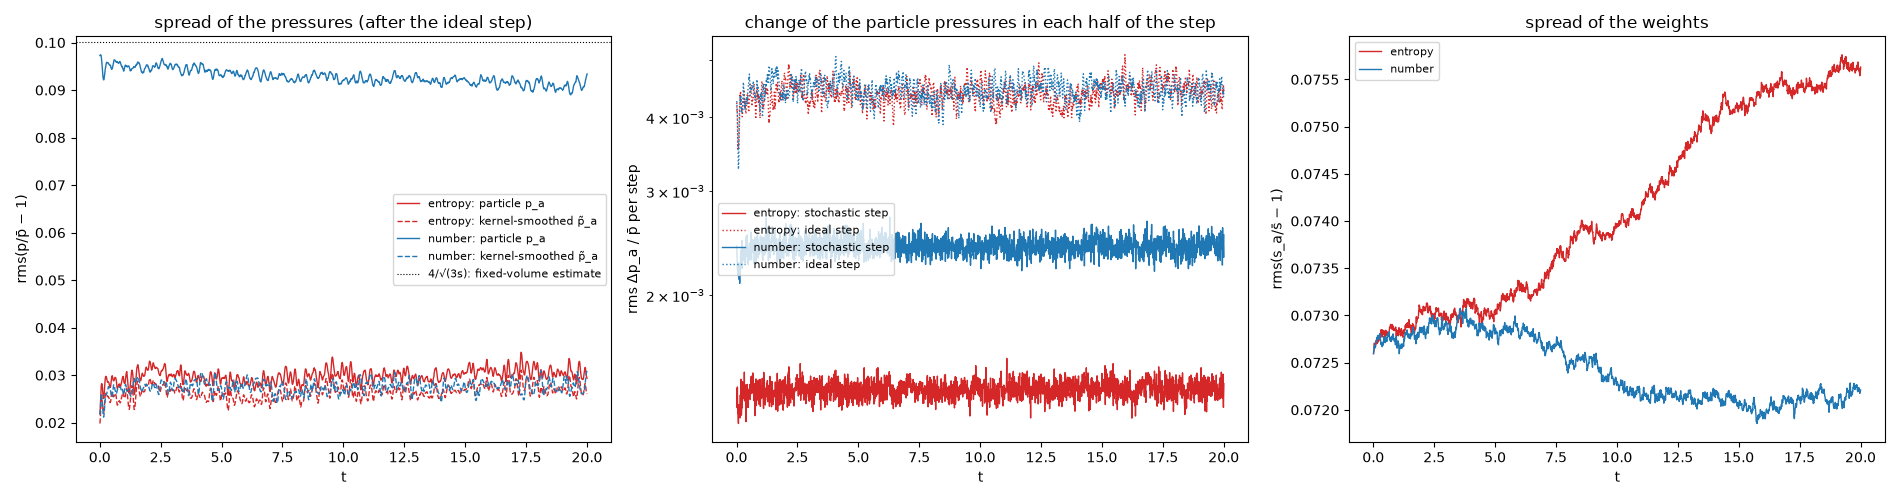
\includegraphics[width=\textwidth]{figs/volume_n_pressure.png}
\caption{Entropy volume (red) and number volume (blue), mean of 2 runs.  Left: spread of the
particle pressures (solid) and of the kernel-smoothed pressures (dashed), after each ideal
step; dotted, the fixed-volume estimate $4/\sqrt{3s}$.  Middle: rms change of the particle
pressures in the stochastic step (solid) and in the ideal step (dotted).  Right: spread of
the weights $s_a$.}
\label{fig:pressure}
\end{figure}

%=============================================================================
\section{Campaign \texttt{volume\_n}}
\label{sec:campaign}

\texttt{nersc/campaign\_volume\_n.txt}, all with \texttt{SPH\_HAMILTONIAN=energy},
\texttt{SPH\_VOLUME=number}, $h/a=2$, $\eta/s=0.2$; packed on one node
(\texttt{nersc/node.sh}, 2 cores per run, 100 runs).  Each set has a counterpart with
the entropy volume from campaigns \texttt{energy2} and \texttt{frozen}.
\begin{center}
\begin{tabular}{lllll}
\hline
set & runs & box, time & $S_0$ ($\delta v$) & tests \\ \hline
\texttt{n\_dt1}, \texttt{n\_dt0.5} & 8+8 & $0.6$, $100$ & $10^6$ ($0.043$) & $H(t)$; $\Delta t$ dependence \\
\texttt{n\_cold} & 4 & $0.6$, $100$ & $10^6$ & thermalization from rest \\
\texttt{n\_ref}, \texttt{n\_s3e5}, \texttt{n\_s1e5} & 16 each & $0.6$, $200$ & $10^6$, $3\times10^5$, $10^5$ & stability, KE, $H$ \\
\texttt{n\_e6}, \texttt{n\_e7} & 16 each & $1.2$, $200$ & $10^6$, $10^7$ ($0.014$) & $C_T$, pair separation \\
\hline
\end{tabular}
\end{center}
Expected: $H$ conserved up to the floor of the ideal step; KE/eq $=1$ at all three
temperatures (no cooling); $C_T$ unchanged; the spreads of $s$ and $V$ show whether the
entropy per particle stays near its thermal spread or walks away.

%=============================================================================
\section{Results}
\label{sec:results}

All 100 runs finished (one node, 21 minutes).  Script
\texttt{examples/volume\_n\_analysis.jl}; the entropy-volume references are campaigns
\texttt{energy2} and \texttt{frozen}.

\paragraph{1. Energy: the steady loss is gone; what is left is a time-step error},
\Fig{fig:vnH}.  At $L=0.6$, $\delta v=0.043$:
\st
-\frac1H\frac{dH}{dt}=\begin{cases}
3.45\times10^{-5} & \text{entropy volume, any }\Delta t,\\
-3.07\times10^{-6} & \text{number volume, }\Delta t,\\
-1.54\times10^{-6} & \text{number volume, }\Delta t/2 .
\end{cases}
\stp
With the number volume $H$ rises slowly, eleven times slower than the entropy volume
loses it, and the rate halves with $\Delta t$: a first-order error of the splitting,
which vanishes as $\Delta t\to0$.  The loss with the entropy volume did not depend on $\Delta t$.  The cold
start reaches KE/eq $=1$ by $t\approx1$ and then drifts like the equilibrium start.
\begin{figure}[t]
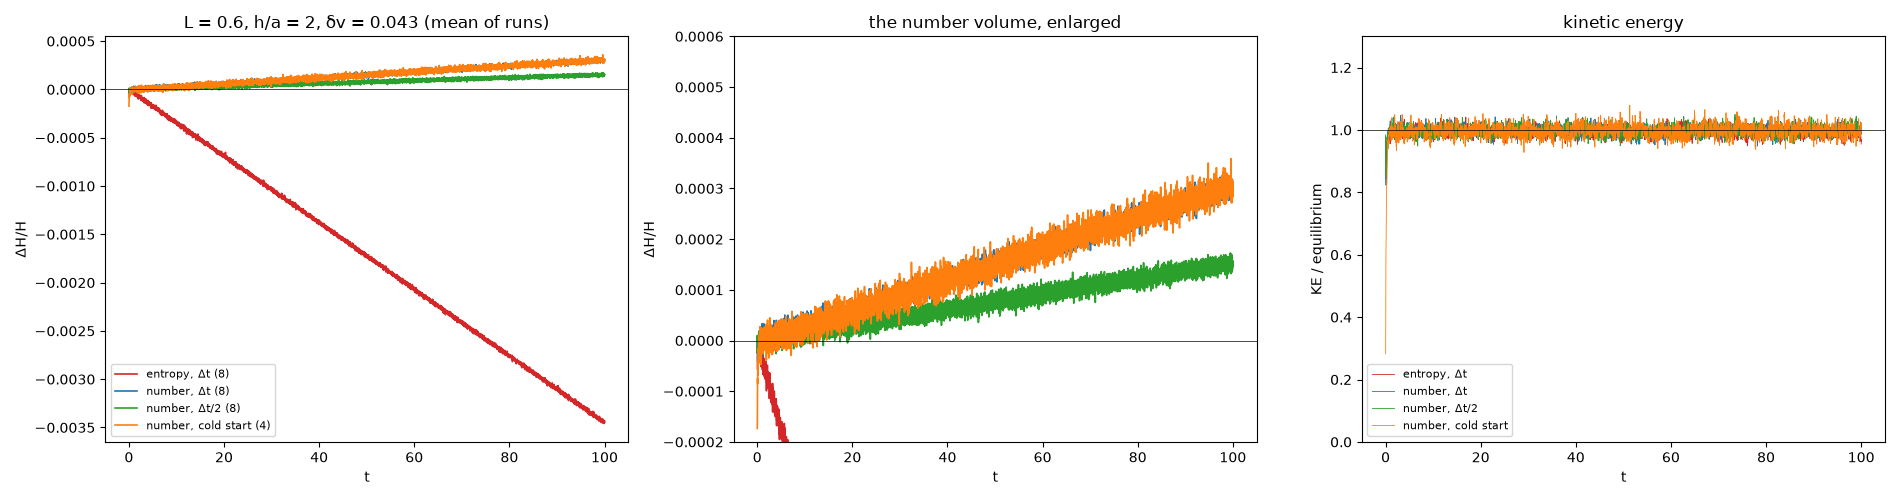
\includegraphics[width=\textwidth]{figs/volume_n_H.png}
\caption{$L=0.6$, $h/a=2$, $\delta v=0.043$.  Left: $\Delta H/H$ against $t$, entropy volume
(red) and number volume at $\Delta t$, $\Delta t/2$ and from a cold start (mean of 8, 8, 4
runs).  Middle: the number volume enlarged.  Right: KE/eq.}
\label{fig:vnH}
\end{figure}

\paragraph{2. Stability: the temperature is held}, \Fig{fig:vnstab}.  The scan of
\texttt{energy2}, 16 runs per point, $t=200$:
\begin{center}
\begin{tabular}{lcccc}
\hline
$\delta v$ & \multicolumn{2}{c}{KE/eq} & \multicolumn{2}{c}{$\Delta H/H$} \\
 & entropy & number & entropy & number \\ \hline
$0.043$ & $0.986$ & $0.985$ & $-0.8\%$ & $+0.06\%$ \\
$0.078$ & $0.812$ & $1.008$ & $-15\%$ & $+0.57\%$ \\
$0.136$ & $0.606$ & $1.020$ & $-31\%$ & $+3.8\%$ \\
\hline
\end{tabular}
\end{center}
No run blows up.  With the number volume the kinetic energy stays at its equilibrium
value at all three temperatures, and $H$ changes by $3.8\%$ at most, where the entropy
volume lost $31\%$.  The remaining heating grows as about $\delta v^{3.6}$; by item 1 it
should fall with $\Delta t$.
\begin{figure}[t]
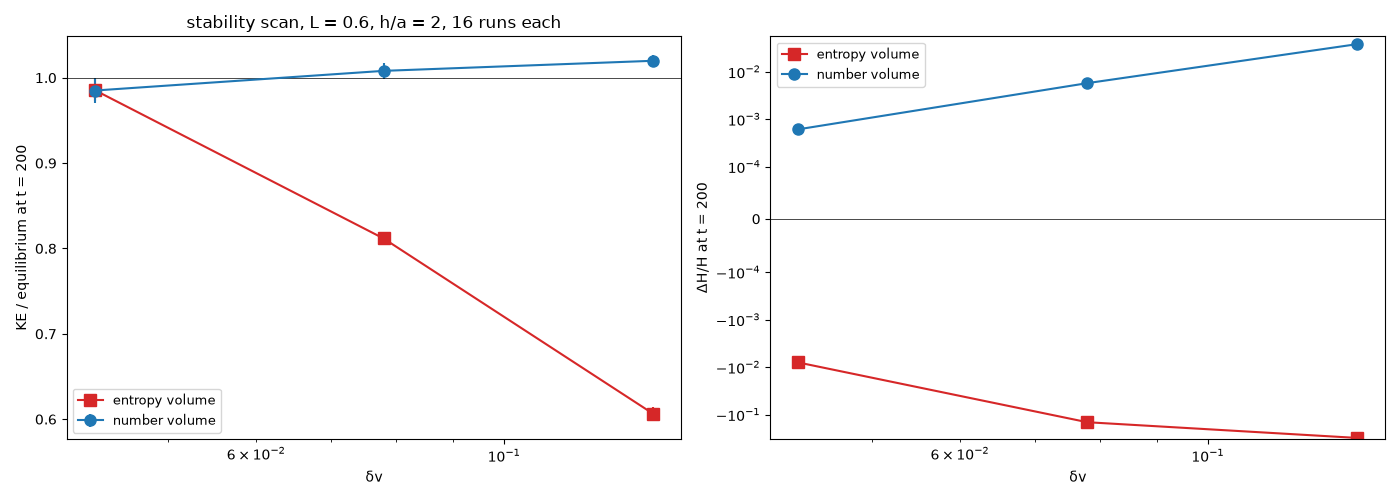
\includegraphics[width=\textwidth]{figs/volume_n_stability.png}
\caption{Stability scan.  Left: KE/eq at $t=200$ against $\delta v$ (mean $\pm$ s.e.).
Right: $\Delta H/H$ at $t=200$ (symmetric log scale): the entropy volume loses energy, the
number volume gains a little.}
\label{fig:vnstab}
\end{figure}

\paragraph{3. The entropy per particle}, \Fig{fig:vnspread}.  From the equilibrium start the
spread of the weights stays at the fixed-volume value $\sqrt{3/s_a}$ ($7.45\%$ at $S_0=10^6$,
$2.36\%$ at $10^7$) and creeps up slowly: from $7.41$ to $7.72\%$ by $t=200$ at $L=1.2$.
From the cold start (all weights equal) it grows like a random walk,
$\mathrm{rms}^2\approx2.1\times10^{-5}\,t$, and reaches $4.6\%$ by $t=100$, still below
$\sqrt{3/s_a}$.  So the weights do not run away to the broad fixed-pressure distribution
of \Sect{sec:thermo} on these times: after the fixed-volume spread is reached the growth
slows tenfold ($\mathrm{rms}^2$ grows by $2.4\times10^{-6}$ per unit time).  Whether it
saturates needs longer runs.  The volumes $1/n_a$, equal on the lattice at the start, spread
by $3.3\%$ ($S_0=10^6$) and $1.0\%$ ($10^7$), in proportion to $\delta v$: the arrangement
is disordered by about half the spread of the entropy per particle.
\begin{figure}[t]
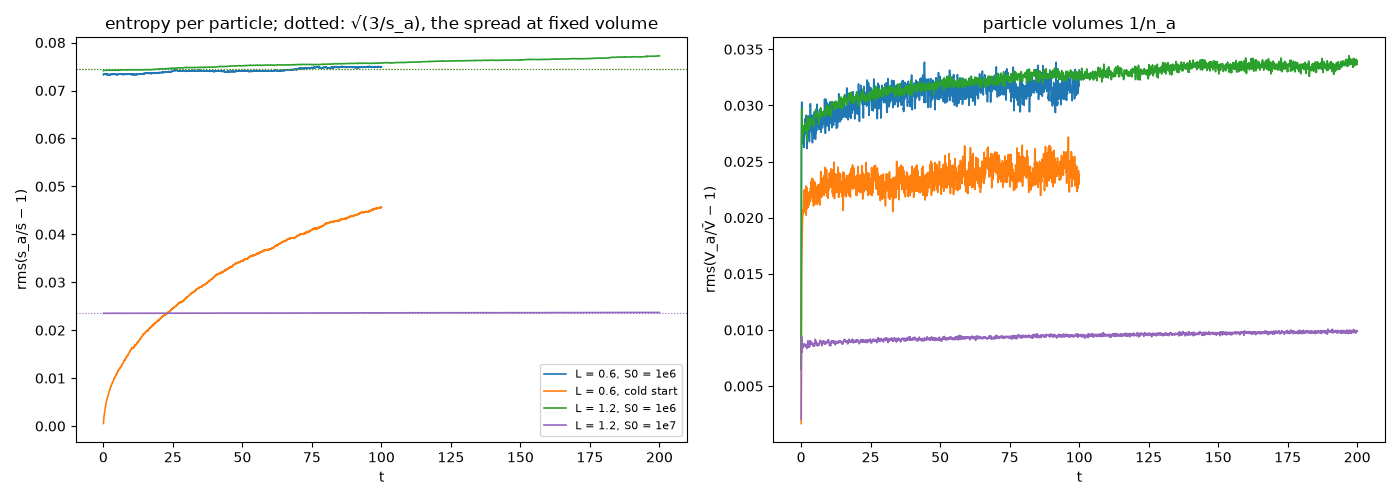
\includegraphics[width=\textwidth]{figs/volume_n_spread.png}
\caption{Number volume.  Left: $\mathrm{rms}(s_a/\bar s-1)$ against $t$ (mean of the runs;
dotted, $\sqrt{3/s_a}$).  Right: $\mathrm{rms}(V_a/\bar V-1)$.}
\label{fig:vnspread}
\end{figure}

\paragraph{4. Correlators and pair separation are unchanged}, \Fig{fig:vnCT} and
\Fig{fig:vnD2}.  At $L=1.2$, 16 runs per set, the transverse correlator is the fluid one with
either volume: $c_t\le0.0025$, $C_T(k,0)/(NVwT)=0.96$--$1.13$, the damping
$2\gamma/\nu k^2=0.7$--$1.3$.  The separation of neighbours is the same to $1\%$:
$D_{\rm rel}(a)=4.03\times10^{-4}$ against $4.04\times10^{-4}$ at $S_0=10^6$, and
$4.03\times10^{-5}$ against $4.08\times10^{-5}$ at $10^7$.  As \Sect{sec:thermo} expects, the
extra mode lives in the arrangement and does not show in $C_T$.
\begin{figure}[t]
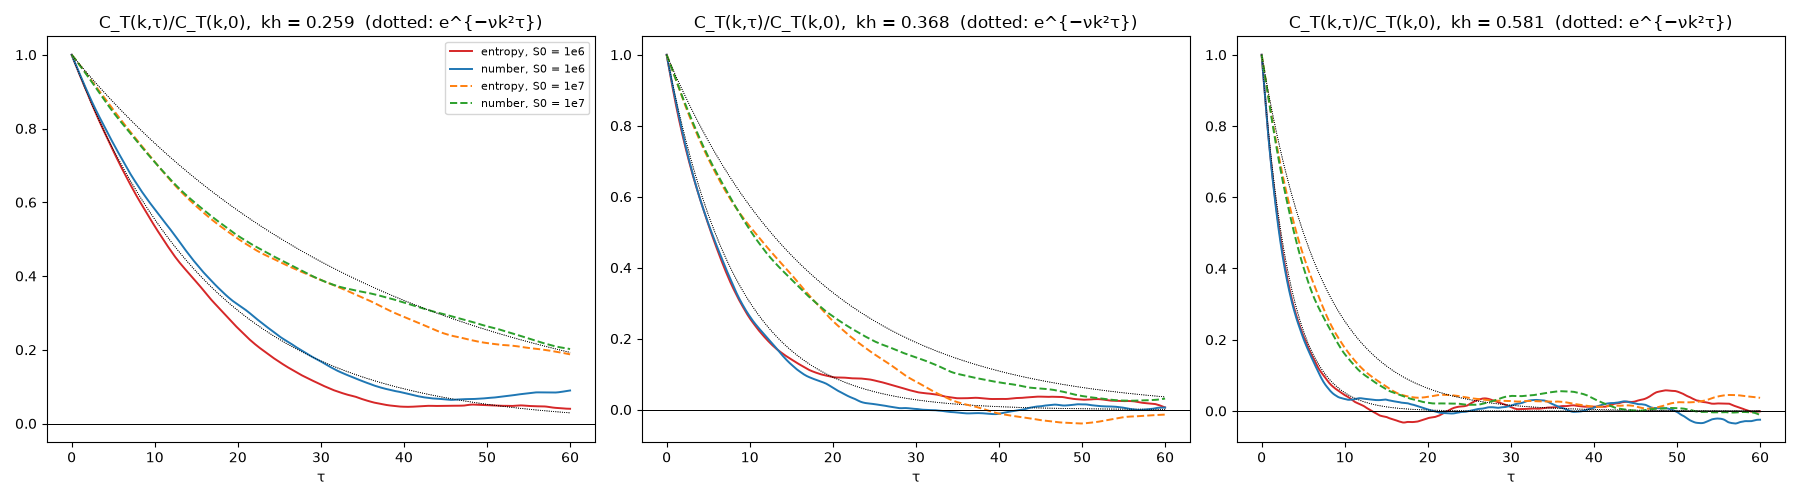
\includegraphics[width=\textwidth]{figs/volume_n_CT.png}
\caption{$C_T(k,\tau)/C_T(k,0)$ at $L=1.2$ in three shells: entropy volume (red, orange) and number
volume (blue, green) at $S_0=10^6$ (solid) and $10^7$ (dashed); dotted, $e^{-\nu k^2\tau}$ for
each $S_0$.}
\label{fig:vnCT}
\end{figure}
\begin{figure}[t]
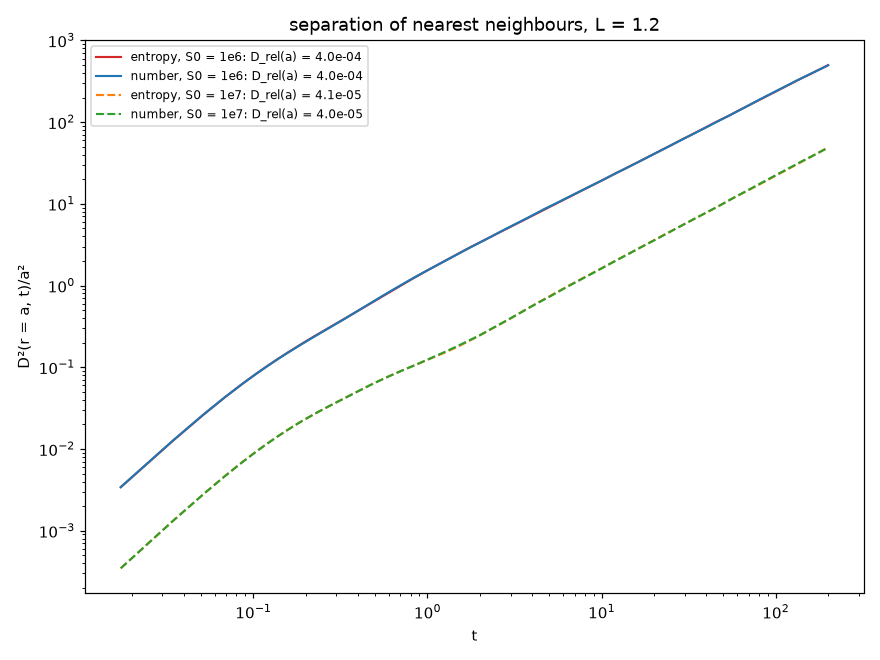
\includegraphics[width=0.6\textwidth]{figs/volume_n_D2.png}
\caption{Separation of nearest neighbours $D^2(a,t)/a^2$, $L=1.2$; the two volumes lie on top
of each other.}
\label{fig:vnD2}
\end{figure}

%=============================================================================
\section{Conclusions}
\label{sec:concl}

\begin{enumerate}
\item The steady loss of energy with \texttt{:energy} came from the back map of the
  stochastic step: the entropy volume moves when the weights change.  The estimate
  \Eq{estimate} follows it step by step.
\item With the number volume $V_a=1/n_a$ the back map is exact.  The loss is gone; what
  remains is a small gain that is first order in $\Delta t$.  The temperature is held up to
  $\delta v=0.136$, where the entropy volume lost $40\%$ of its kinetic energy.
\item The price is a particle-scale pressure noise at the level of a fluid cell of volume
  $V_a$, and a disorder of the volumes of half the spread of the entropy per particle.
  Neither shows on the scale of the kernel: the smoothed pressures, $C_T$ and the pair
  separation are the same as with the entropy volume.
\item The entropy per particle behaves as a passive charge.  On the times run it stays near
  its fixed-volume spread and creeps slowly; it does not run away.
\end{enumerate}

\paragraph{Next.}  (a) The remaining first-order heating: a symmetric splitting of the
stochastic step.  (b) Longer runs for the spread of the entropy per particle.  (c) The
deterministic tests with the number volume (\texttt{number\_tests.tex}).  (d) With the owner,
whether to make \texttt{SPH\_VOLUME=number} the default with \texttt{:energy}.

\end{document}
